Every country has its nominal frequency of the oscillations of alternating current in an electric power grid transmitted from a power station to the end-user. For instance, the nominal value is 50Hz \cite{papadopoulos2009distribution} in the UK while it’s 60Hz \cite{komarnicki2008practical} in USA.\\

However, \cite{machowski2011power} if a load is suddenly connected or disconnected to the system, or if the protection equipment suddenly disconnects a generating, there be a distortion in the power balance between that delivered by the turbines and that consumed by the loads. This imbalance is initially covered from \cite{machowski2011power} the kinetic energy of rotating rotors of turbines, generators and motors and, as a result, the frequency in the system change.\\

If there is a mismatch between the generation and the demand, for instance, due to the outage of one generating unit, then the frequency starts to drop down.  \\

If no control is applied, the frequency will largely deviates and then reaches a meagre and steady-state value, due to which the electrical grid is shut down.\\

\begin{figure}[t]
\center
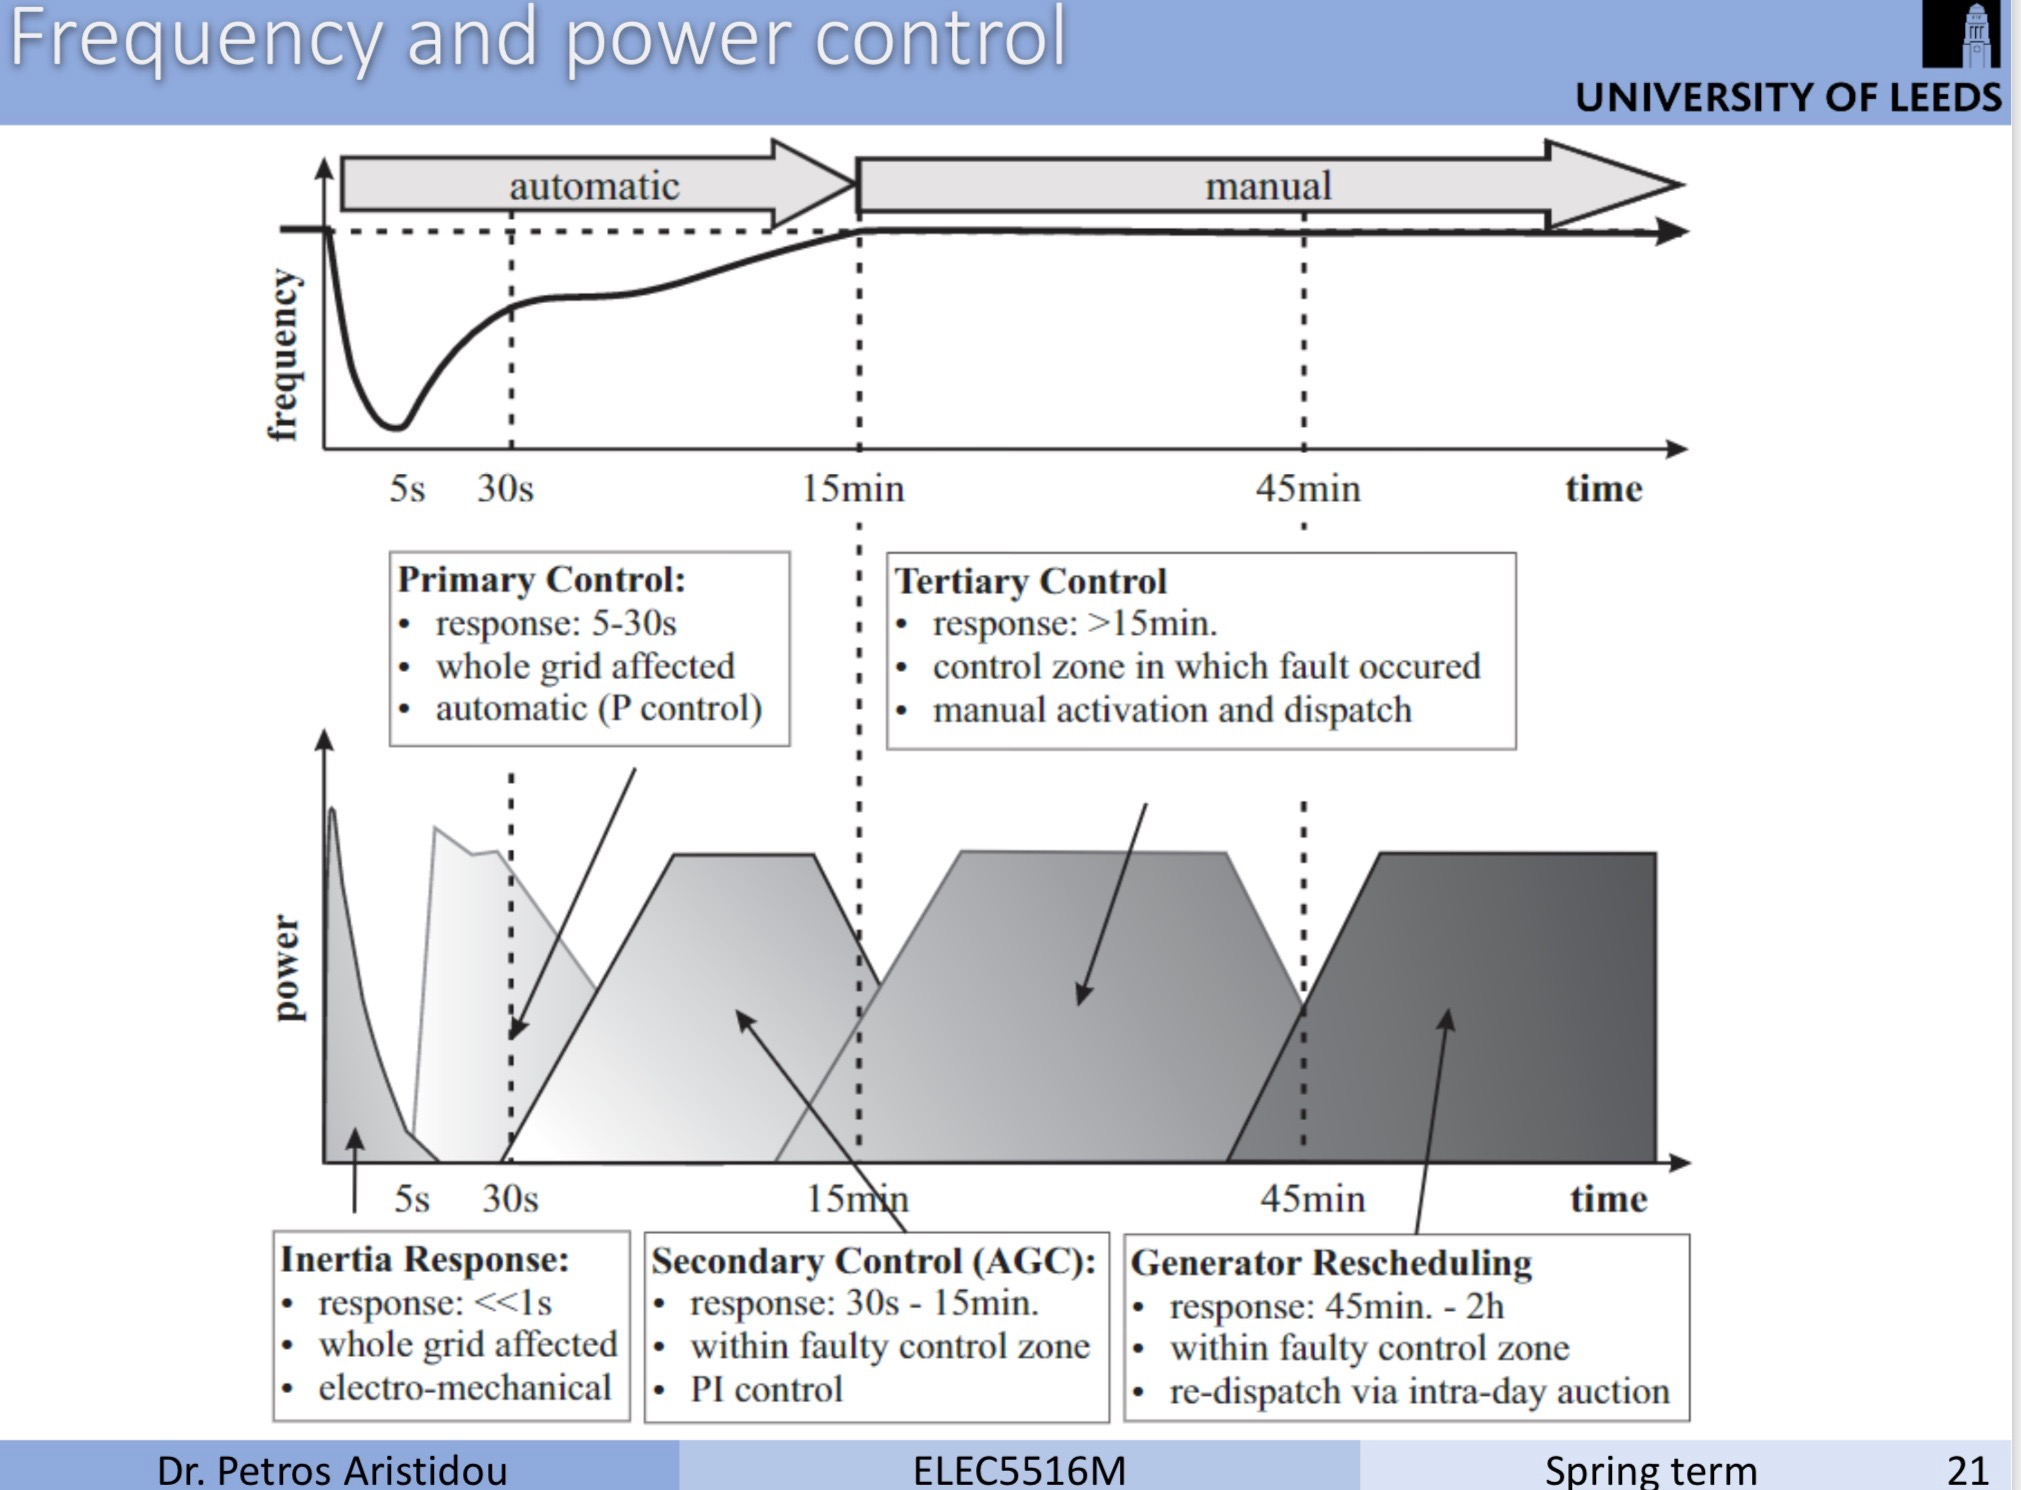
\includegraphics[scale=0.2]{figure/2_1_freq.jpeg}
\caption{Frequency and power control.}
\label{2_1_freq}
\end{figure}

The mechanism of primary frequency control is to restore the active power balance in a power system. After primary control takes place, the power balance is restored at a lower or higher frequency. Normally it takes seconds and responses from 5 seconds to 30 seconds. It is a partly Automatic Generation Control.\\


However, the frequency does not go back to its nominal value and remains at a steady-state value below or above the nominal one. To avoid damages to equipment and loads, we need secondary frequency control to \cite{machowski2011power} restore the frequency balance to its nominal value or to eliminate the steady-state error/frequency error. Normally it takes minutes and responses from 30 seconds to 15 minutes. It is a fully Automatic Generation Control.\\


Tertiary Frequency Control encompasses actions taken to capture current and future emergencies by getting resources. Alternate deployment and recovery after a disturbance are common types of Tertiary Control. Normally it takes dozens of minutes and responses longer than 15 minutes. It is a fully manual control.